% SC4012 --- Chapter 4: Crypto Misuse (0->100 ground-up)
\chapter{Cryptographic Misuse: TLS, Padding Oracles and Side Channels}
\label{ch:crypto-misuse}

\begin{quote}
\emph{``Cryptography is easy to use incorrectly and hard to notice.''} --- Correct primitives with wrong composition, missing checks, or leaky implementations break just as badly as no crypto at all.
\end{quote}

\noindent\fbox{\parbox{\dimexpr\linewidth-2\fboxsep-2\fboxrule}{%
\textbf{From zero: what crypto promises.} We assume no prior crypto. We build from ``what TLS does on the wire,'' through a padding-oracle that decrypts without the key, to timing leaks that steal keys through the clock. Every failure is a misuse, not a broken primitive.}}
\vspace{0.4em}

\section*{Learning Outcomes}
After this chapter you will be able to:
\begin{enumerate}[label=(L\arabic*)]
    \item sketch the TLS 1.3 handshake and what each message proves;
    \item explain padding-oracle and why MAC-then-encrypt plus distinct errors breaks;
    \item describe timing and cache side channels and constant-time defences;
    \item identify misuse patterns (ECB, IV reuse, hard-coded keys, bad randomness);
    \item select AEAD, certificate validation, and HSTS as safe defaults.
\end{enumerate}

% ============================================================
\section{TLS: What It Is Supposed to Do}
\label{sec:tls}
Intuition: Alice wants to talk to \texttt{bank.com} over a network the attacker controls. She needs three things: (i) the server is who it claims, (ii) nobody can read or change messages, (iii) replay or downgrade is detected. TLS provides all three by composing authentication (certificates/PKI), key exchange (ECDHE), and authenticated encryption (AEAD).

\begin{figure}[h]\centering
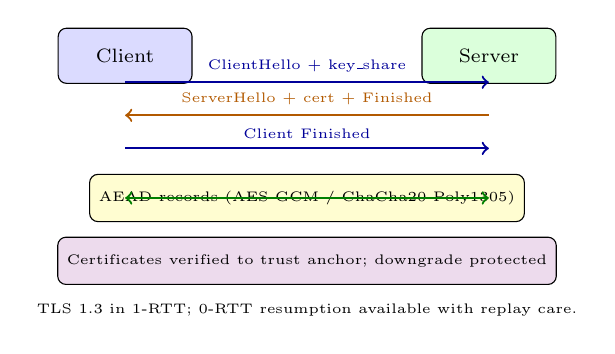
\begin{tikzpicture}[scale=0.84,every node/.style={font=\scriptsize}]
  \node[draw,fill=blue!14,rounded corners=3pt,minimum width=1.7cm,minimum height=0.7cm,align=center] (c) at (0,3.0) {Client};
  \node[draw,fill=green!14,rounded corners=3pt,minimum width=1.7cm,minimum height=0.7cm,align=center] (s) at (5.5,3.0) {Server};
  \draw[->,thick,blue!60!black] (0,2.6) -- (5.5,2.6) node[midway,above,font=\tiny] {ClientHello + key\_share};
  \draw[<-,thick,orange!70!black] (0,2.1) -- (5.5,2.1) node[midway,above,font=\tiny] {ServerHello + cert + Finished};
  \draw[->,thick,blue!60!black] (0,1.6) -- (5.5,1.6) node[midway,above,font=\tiny] {Client Finished};
  \node[draw,fill=yellow!18,rounded corners=3pt,minimum width=3.4cm,minimum height=0.6cm,align=center,font=\tiny] at (2.75,0.85) {AEAD records (AES-GCM / ChaCha20-Poly1305)};
  \draw[<->,thick,green!50!black] (0,0.85) -- (5.5,0.85);
  \node[draw,fill=violet!14,rounded corners=3pt,minimum width=5.0cm,minimum height=0.6cm,align=center,font=\tiny] at (2.75,-0.1) {Certificates verified to trust anchor; downgrade protected};
  \node[font=\tiny,align=center] at (2.75,-0.85) {TLS 1.3 in 1-RTT; 0-RTT resumption available with replay care.};
\end{tikzpicture}
\caption{TLS 1.3 handshake (abstract). Certificates authenticate the server, (EC)DHE provides forward secrecy, and the Finished MACs bind the transcript so no message can be altered or rolled back.}
\label{fig:tls-handshake}
\end{figure}

\begin{definition}[TLS guarantees]
After a successful handshake with valid certificate chain, the client and server share a fresh AEAD session key. Every record is confidential (ciphertext hides plaintext), authenticated (tampering is detected), and replay/downgrade protected (transcript is MAC'd). Failure to check any of these (e.g., skipping cert validation) voids the guarantee.
\end{definition}

Typical misuse: disabling certificate validation for development and shipping it, or using TLS without HSTS so the first connection can be downgraded to HTTP. The wire is then encrypted to the wrong party.

\begin{lstlisting}[language=Python]
# Python: correct cert validation is the default -- keep it
import ssl, socket
ctx = ssl.create_default_context()  # loads CA bundle, checks hostname
# NEVER do: ctx.check_hostname = False; ctx.verify_mode = ssl.CERT_NONE
with socket.create_connection(("bank.com", 443)) as sock:
    with ctx.wrap_socket(sock, server_hostname="bank.com") as tls:
        tls.sendall(b"GET / HTTP/1.0\r\n\r\n")
        print(tls.recv(4096))
\end{lstlisting}

Forward secrecy (ECDHE) means compromise of the long-term key does not decrypt past sessions; RSA key transport (old) does not have this property and is removed in TLS~1.3. Session resumption with 0-RTT saves a round trip but replays the first message; servers must make 0-RTT requests idempotent or reject them for non-idempotent actions (e.g., POST).

 of the long-term key does not decrypt past sessions; RSA key transport (old) does not have this property and is removed in TLS~1.3.

% ============================================================
\section{Padding Oracles: Decrypting Without the Key}
\label{sec:padding-oracle}
TLS~1.0 used MAC-then-encrypt with CBC and PKCS\#7 padding. The server returned distinct errors for ``bad MAC'' vs.\ ``bad padding.'' Vaudenay (2002) showed that distinction is a decryption oracle.

\begin{definition}[Padding oracle]
A \emph{padding oracle} answers whether a ciphertext's plaintext has valid padding. With CBC, flipping a byte in block $C_{i-1}$ flips the same byte in the padding of $P_i$ after decryption, letting the attacker learn $P_i$ byte-by-byte by observing the oracle's answer.
\end{definition}

\begin{figure}[h]\centering
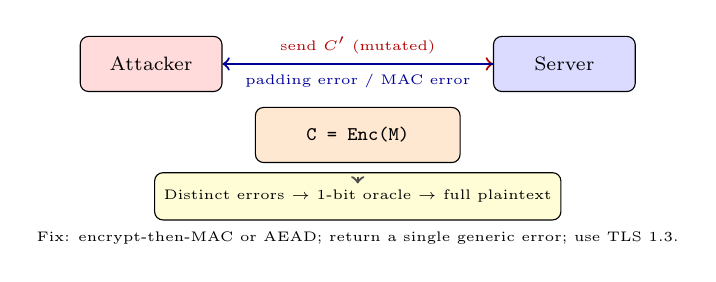
\begin{tikzpicture}[scale=0.82,every node/.style={font=\scriptsize}]
  \node[draw,fill=red!14,rounded corners=3pt,minimum width=1.8cm,minimum height=0.7cm,align=center] (atk) at (-3.2,1.5) {Attacker};
  \node[draw,fill=blue!14,rounded corners=3pt,minimum width=1.8cm,minimum height=0.7cm,align=center] (srv) at (3.2,1.5) {Server};
  \node[draw,fill=orange!18,rounded corners=3pt,minimum width=2.6cm,minimum height=0.7cm,align=center] (c) at (0,0.4) {\texttt{C = Enc(M)}};
  \draw[->,thick,red!70!black] (atk) -- (srv) node[midway,above,font=\tiny] {send $C'$ (mutated)};
  \draw[<-,thick,blue!60!black] (atk) -- (srv) node[midway,below,font=\tiny] {padding error / MAC error};
  \node[draw,fill=yellow!16,rounded corners=3pt,minimum width=4.2cm,minimum height=0.6cm,align=center,font=\tiny] at (0,-0.55) {Distinct errors $\to$ 1-bit oracle $\to$ full plaintext};
  \draw[->,thick,gray!60!black,dashed] (0,-0.25) -- (0,-0.35);
  \node[font=\tiny,align=center] at (0,-1.2) {Fix: encrypt-then-MAC or AEAD; return a single generic error; use TLS~1.3.};
\end{tikzpicture}
\caption{Padding-oracle attack. The attacker mutates ciphertext and learns from the server's error message which padding was valid, iterating to recover the plaintext without the key.}
\label{fig:padding-oracle}
\end{figure}

Fixes: use AEAD (AES-GCM, ChaCha20-Poly1305) where padding is not needed; if CBC must remain, use encrypt-then-MAC and a uniform error message plus constant-time padding check. TLS~1.3 removes the vulnerable construction entirely.

\begin{lstlisting}[language=Python]
# Misuse: home-made MAC-then-encrypt with distinct errors (DON'T)
def decrypt_and_check(ciphertext):
    pt = aes_cbc_decrypt(key, ciphertext)
    if not valid_pkcs7(pt):  raise PaddingError("pad")   # oracle!
    if not hmac_verify(pt):  raise MacError("mac")       # distinct
    return pt
# Safe: use an AEAD library; one error, constant time
# from cryptography.hazmat.primitives.ciphers.aead import AESGCM
# AESGCM(key).decrypt(nonce, ciphertext, associated_data)
\end{lstlisting}

The same pattern appears outside TLS: XML padding oracles (Vaudenay-style on CBC-encrypted SAML tokens), JWT \texttt{alg: none} or \texttt{alg: HS256} confusion where an RSA public key is misused as an HMAC secret, and any API that says ``invalid padding'' vs.\\ ``invalid token'' leaks the same bit. The defence is always: one generic error, constant time, and a vetted AEAD.

 XML padding oracles, JWT alg confusion, and any API that says ``invalid padding'' vs.\ ``invalid token'' leaks the same bit.

% ============================================================
\section{Side Channels: Keys Leaking Through Time and Cache}
\label{sec:side-channels}
A side channel leaks a secret through a non-functional property: how long a computation took, how much power it drew, or which cache lines were accessed. The implementation is correct functionally but not constant-time.

\begin{definition}[Timing/cache side channel]
A \emph{timing side channel} exists when execution time depends on secret data (e.g., early exit on MAC mismatch, table lookup indexed by key). A \emph{cache side channel} (Flush+Reload, Prime+Probe) infers a victim's memory accesses by observing cache contention.
\end{definition}

\begin{figure}[h]\centering
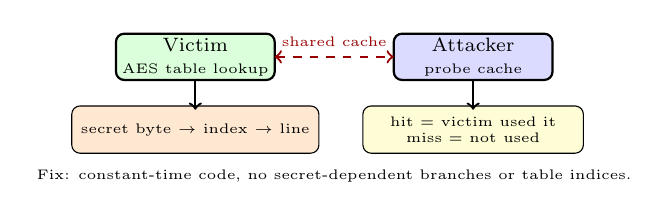
\begin{tikzpicture}[scale=0.84,every node/.style={font=\scriptsize}]
  \draw[thick,fill=green!14,rounded corners=3pt] (0,1.6) rectangle (2.4,2.3) node[midway,align=center] {Victim\\ \tiny AES table lookup};
  \draw[thick,fill=blue!14,rounded corners=3pt] (4.2,1.6) rectangle (6.6,2.3) node[midway,align=center] {Attacker\\ \tiny probe cache};
  \draw[<->,thick,red!60!black,dashed] (2.4,1.95) -- (4.2,1.95) node[midway,above,font=\tiny] {shared cache};
  \node[draw,fill=orange!18,rounded corners=3pt,minimum width=2.8cm,minimum height=0.6cm,align=center,font=\tiny] at (1.2,0.85) {secret byte $\to$ index $\to$ line};
  \node[draw,fill=yellow!16,rounded corners=3pt,minimum width=2.8cm,minimum height=0.6cm,align=center,font=\tiny] at (5.4,0.85) {hit = victim used it\\miss = not used};
  \draw[->,thick] (1.2,1.6) -- (1.2,1.15); \draw[->,thick] (5.4,1.6) -- (5.4,1.15);
  \node[font=\tiny,align=center] at (3.3,0.15) {Fix: constant-time code, no secret-dependent branches or table indices.};
\end{tikzpicture}
\caption{Cache side channel. The victim's secret-dependent table access loads a cache line; the attacker times its own accesses to learn which line was loaded, inferring the secret.}
\label{fig:cache-channel}
\end{figure}

Constant-time means no branches on secrets, no memory accesses indexed by secrets, and no variable-time instructions (early-exit compare, division). Libraries that get this right (NaCl, BoringSSL) use bit-sliced AES or AES-NI, constant-time compares, and blinding for RSA.

\begin{example}[Lucky13 and string compare]
Fixing Lucky13 required uniform error timing plus constant-time MAC verification; the same lesson applies to any API that returns early on failure. A modern AEAD API that returns a single boolean and is implemented in constant time removes the entire class.

\end{example}

\begin{example}[Lucky13 detail]
TLS CBC timing (Lucky13, 2013) distinguished MAC check time from padding check time, recreating the padding oracle via timing. Similarly, \texttt{memcmp(secret, guess)} that returns on first mismatch leaks the prefix length; \texttt{CRYPTO\_memcmp} (constant-time) fixes it.
\end{example}

% ============================================================
\section{Randomness, Keys and Custom Crypto}
\label{sec:keys-rand}
Keys must be random and secret; nonces must be unique. Using \texttt{rand()} (predictable), \texttt{time()} as seed, or EC-DSA with repeated $k$ leaks the private key directly (Sony PS3, 2010). Hard-coded keys in binaries are extracted in minutes with \texttt{strings} or Ghidra. Store keys in an HSM/KMS, rotate them, and never log them.

Custom crypto (``we XOR with a secret constant'') is almost always broken: it lacks peer review, has no reduction to a hard problem, and fails at composition. Use vetted AEAD and key-derivation (HKDF, Argon2 for passwords); the only correct answer to ``should we design our own cipher'' is no.

\begin{remark}[Password storage done right]
Passwords need a slow, salted hash (Argon2, bcrypt, scrypt), not fast SHA-256. Each password gets a unique salt and a work factor tuned to $\sim$100\,ms. Fast hashes let an attacker test billions of guesses per second; a slow hash with salt forces per-password work and defeats rainbow tables.
\end{remark}

% ============================================================
\section{Certificate Validation and HSTS}
\label{sec:cert-hsts}
TLS without correct validation is plaintext to an active attacker. The client must: (i) verify the chain to a trust anchor, (ii) check hostname matches, (iii) check validity period and revocation (CRL/OCSP), (iv) reject short keys and weak hashes. Libraries that make ``insecure'' mode easy (\texttt{-k} in curl, \texttt{verify\_mode=CERT\_NONE}) invite misuse; safe wrappers should require an explicit, audited exception.

HSTS (\texttt{Strict-Transport-Security}) tells the browser to never use HTTP for this origin, removing the first-visit downgrade that enables SSL-stripping. Preload lists and \texttt{includeSubDomains} extend the guarantee. For internal services, pin certificates or use mutual TLS.

% ============================================================
\section{Misuse Checklist}
\label{sec:misuse-checklist}
Common misuse catalogue, each with a one-line detector: ECB mode (deterministic, leaks patterns; grep \texttt{MODE\_ECB} or check for repeated ciphertext blocks), IV/nonce reuse (GCM breaks catastrophically; grep for constant \texttt{nonce} or counter reset), hard-coded keys in binaries (\texttt{strings | grep key}), weak randomness (\texttt{rand()} instead of \texttt{getrandom} / \texttt{BCryptGenRandom}), and custom crypto (``we designed our own cipher''; require review).

 (deterministic, leaks patterns), IV/nonce reuse (GCM breaks catastrophically), hard-coded keys in binaries, weak randomness (\texttt{rand()} instead of \texttt{getrandom}), and custom crypto (``we designed our own cipher'').

Safe defaults: AEAD with random nonce (96-bit, never reuse), TLS~1.3 with default context, X.509 validation enabled, HSTS (\texttt{Strict-Transport-Security}), certificate transparency, and a randomness source from the OS (\texttt{getrandom} / \texttt{/dev/urandom}). Anything else needs a written justification and review. Checklists for audits: grep for \texttt{MODE\_ECB}, \texttt{CERT\_NONE}, \texttt{rand()}, hard-coded \texttt{key=}, and missing tag checks, TLS~1.3 with default context, X.509 validation enabled, HSTS (\texttt{Strict-Transport-Security}), certificate transparency, and a randomness source from the OS. Anything else needs a written justification and review.

% ============================================================
\section{Composing Primitives Safely}
\label{sec:compose-crypto}
Composition is where misuse concentrates. Encrypt-then-MAC, or better a single AEAD, is safe; MAC-then-encrypt and encrypt-and-MAC are fragile. Key separation (different keys for different purposes, derived via HKDF with distinct \texttt{info} strings) prevents cross-protocol attacks where a ciphertext from one context is accepted in another. Always bind context (associated data) into the AEAD so a ciphertext cannot be transplanted.


\begin{remark}[Checklist for reviewers]
When reviewing crypto code, check: (1) is the library vetted (BoringSSL, libsodium) and not home-rolled? (2) are nonces unique (and 96-bit for GCM)? (3) is validation enabled and hostname checked? (4) are errors uniform and constant-time? (5) are keys from a CSPRNG and stored in a KMS? A ``yes'' to all five prevents the majority of CVEs tagged ``crypto misuse.''
\end{remark}


\begin{example}[JWT alg confusion]
A server verifies JWT with \texttt{verify(token, key)} where \texttt{key} is the RSA public key when \texttt{alg} is \texttt{RS256}, but the attacker sets \texttt{alg} to \texttt{HS256} and signs with HMAC using the public key bytes as the symmetric secret. The server then checks HMAC with the same bytes and accepts the forged token. Fix: allow-list expected algs and use distinct keys per alg.
\end{example}


\begin{remark}[Why TLS 1.3 removed the sharp edges]
TLS~1.3 removed RSA key transport, CBC+MAC-then-encrypt, compression, and renegotiation --- each had been the root cause of a major attack (Bleichenbacher, Lucky13, CRIME, Triple Handshake). Fewer options mean fewer misuses; the lesson for application crypto is the same: expose one safe AEAD, not five fragile modes.
\end{remark}

% ============================================================
\section{Exercises}
\label{sec:ch04-exercises}
\begin{enumerate}[label=E4.\arabic*, leftmargin=*, itemsep=0.6em]
    \item \textbf{TLS downgrade.} Explain how an attacker who can intercept the first HTTP request downgrades a site without HSTS. What does \texttt{Strict-Transport-Security: max-age=63072000; includeSubDomains} prevent, and what attack remains on first visit?
    \item \textbf{Padding oracle by hand.} In CBC, $P_i = D_k(C_i)\oplus C_{i-1}$. If you flip byte $j$ of $C_{i-1}$, which byte of $P_i$ flips and why? Describe how a padding oracle that answers ``valid PKCS\#7 or not'' lets you recover $P_i[15]$ (last byte) in at most 256 queries.
    \item \textbf{Constant-time compare.} Write in Python (or pseudocode) a constant-time equality for two byte strings that always examines every byte and uses no early exit. Explain why a naive \texttt{==} leaks timing and how your fix avoids it.
    \item \textbf{Nonce reuse in GCM.} What breaks if an AES-GCM nonce is reused with the same key? State the concrete forgery or plaintext recovery and the engineering rule that prevents it (counter vs.\ random nonce, 96-bit, never repeat).
    \item \textbf{Audit snippet.} Audit: \texttt{cipher = AES.new(key, AES.MODE\_ECB); ct = cipher.encrypt(pad(msg));}. List three misuses and rewrite using \texttt{AES-GCM} with a random 96-bit nonce, handling associated data and tag verification in one step.
\end{enumerate}

\section*{Chapter Notes}
Vaudenay padding oracles (Eurocrypt~2002); Lucky13 (AlFardan \& Paterson, 2013); BEAST/CRIME/BREACH and POODLE are earlier composition failures. TLS~1.3 is RFC~8446; AEAD is RFC~5116. Side channels surveyed in Kocher (timing, 1996), Bernstein (cache, 2005), and Yarom \& Falkner (Flush+Reload, 2014). Constant-time guidance from Bernstein, Schwabe and the BearSSL/BoringSSL docs.

% End of Chapter 4
